  
\documentclass[letterpaper,aps,prc,superscriptaddress,nofootinbib,10pt,showpacs,floatfix]{revtex4-2}
\usepackage{graphicx}
\usepackage{comment}
\usepackage{setspace}
\usepackage{amsmath}
\usepackage{amssymb}
\usepackage{color}
\usepackage{indentfirst}
\usepackage{xspace}
\usepackage{hyperref}
\usepackage{verbatim}
\usepackage{epstopdf}
\usepackage{hyperref}
\usepackage{placeins}
\usepackage{xfrac}
\usepackage[table]{xcolor}
\usepackage{array}
\usepackage{changepage}
\usepackage{float}
\usepackage{enumitem}

\newcolumntype{P}[1]{>{\centering\arraybackslash}p{#1}}
\newcolumntype{M}[1]{>{\centering\arraybackslash}m{#1}}
\newcommand{\addmathvspace}{\vrule width 0pt height 4ex depth 2.5ex}
\newcommand{\sqs}{\mbox{$\sqrt{s}$}\xspace}
\newcommand{\ee}{\mbox{$e^{+} e^{-}$}\xspace}
\newcommand{\pp}{\mbox{$pp\,(p\bar{p})$ }\xspace}
\newcommand{\bfrac}[2]{\frac{\displaystyle #1}{\displaystyle #2}}

\setlength{\arrayrulewidth}{0.8mm}
\graphicspath{ {./Images/} }



\begin{document}

\title{MEASUREMENT OF THE HIGHER MOMENTS OF TRANSVERSE MOMENTUM OF CHARGED PARTICLES IN PROTON-PROTON COLLISIONS}
\author{Akash Verma}
\email{190260005@iitb.ac.in}
\affiliation{Indian Institute of Technology Bombay, Mumbai, India}
\author{Ankan Mukherjee} 
\email{190260008@iitb.ac.in}
\affiliation{Indian Institute of Technology Bombay, Mumbai, India}
\author{Divyansh Singh Gehlot}
\email{190100047@iitb.ac.in}
\affiliation{Indian Institute of Technology Bombay, Mumbai, India}
\author{Drishti Baruah}
\email{190260019@iitb.ac.in}
\affiliation{Indian Institute of Technology Bombay, Mumbai, India}
\author{Janak Ruia}
\email{190260038@iitb.ac.in}
\affiliation{Indian Institute of Technology Bombay, Mumbai, India}
\author{Mithil Vakde}
\email{mvakde@iitb.ac.in}
\affiliation{Indian Institute of Technology Bombay, Mumbai, India}
\author{Sachin Teli}
\email{190260042@iitb.ac.in}
\affiliation{Indian Institute of Technology Bombay, Mumbai, India}
\author{Vignesh Tongaria}
\email{190260046@iitb.ac.in}
\affiliation{Indian Institute of Technology Bombay, Mumbai, India}
%\email{ashutosh.kumar.pandey@cern.ch}
%\email{sadhana@phy.iitb.ac.in}


\date{\today}  



\maketitle
\vspace{-10mm}
\section*{Abstract}
\vspace{-2mm}
\begin{adjustwidth}{20pt}{20pt}
We aim to analyze p-p collisions by studying the transverse momenta of the ejected particles. We reproduce the results obtained by Giuliano Giacalone, Fernando G. Gardim {\it et al.} in their paper on mean transverse momentum fluctuations in heavy-ion collisions \cite{fluct}. Using the data generated from the Pythia 8 generator, we plot the mean transverse momenta of multiple p-p collisions. We verify the positively skewed deviation of mean transverse momentum $\mathbf{\langle p_T \rangle}$ from Gaussian distribution. First, we divide the data into different multiplicity classes and plot the distribution of $\mathbf{p_T}$ and $\mathbf{\langle  p_T\rangle}$. Then we observe how mean and intensive variance of $\mathbf{p_T}$ change over different multiplicity classes. Finally, we find intensive and standardized skewness of $\mathbf{p_T}$ for different multiplicity classes. 
\end{adjustwidth}
\vspace{-2mm}


\section{Introduction}
\vspace{-2mm}
For a given collision centrality, the mean transverse momentum $\mathbf{\langle  p_T\rangle}$ of emitted particles in ultra-relativistic proton-proton collisions fluctuates from one event to another. The distribution of $\mathbf{\langle  p_T\rangle}$ in event-by-event dynamics reflects the various statistical and dynamical fluctuations.
 
In this project, through various plots, we will show that the probability distribution of $\mathbf{\langle  p_T\rangle}$ is \textbf{not Gaussian} but has \textbf{positive skew}, which arises because of the above-mentioned fluctuations.

We then go on to plot two dimensionless measures of skewness versus different multiplicity classes, namely \textbf{standardized skewness} and \textbf{intensive skewness}, out of which the first depends on centrality and system size, whereas the second has the property of being independent of the system size. Since these are dimensional quantities, both of these are expected to be less sensitive to analysis details,
such as those dependent on the detector.

We shall be using the following definitions as per the \textbf{STAR} collaboration.
\vspace{-1mm}
\begin{equation}
\label{eq:1}
\mathrm{Mean\ Transverse\ Momentum}=\langle \langle p_T\rangle \rangle =\left\langle \bfrac{\Sigma_{i=1}^{N_{ch}} p_i}{N_{ch}}\right\rangle 
\end{equation}

where $N_{ch}$ denotes the number of charged particles in an event, $p_i$ is the transverse momentum of the $i$th particle and angular brackets denote an average over events in a centrality class.

We analyze the variance of dynamical $p_T$ fluctuations which we denote by $\langle \Delta p_i \Delta p_j\rangle $,
\begin{equation}
\label{eq:2}
\langle \Delta p_i \Delta p_j \rangle =\left\langle \bfrac{\Sigma_{i;j\neq i}\ {(p_i-\langle \langle p_T\rangle \rangle )(p_j-\langle \langle p_T\rangle \rangle )}}{N_{ch}(N_{ch}-1)}\right\rangle 
\end{equation}
which can also be written as
\begin{equation}
\label{eq:3}
\langle \Delta p_i \Delta p_j\rangle =\langle \left(\langle p_T\rangle -\langle \langle p_T\rangle \rangle \right)^2\rangle 
\end{equation}
and the intensive variance of transverse momentum which is defined as follows
\begin{equation}
\label{eq:4}
\sigma_{p_T}=\bfrac{\langle \Delta p_i \Delta p_j\rangle ^{\sfrac{1}{2}}}{\langle \langle p_T\rangle \rangle }.
\end{equation}
The skewness is the third central moment, denoted by $\langle \Delta p_i \Delta p_j \Delta p_k\rangle $ defined as follows
\begin{equation}
\label{eq:5}
\langle \Delta p_i \Delta p_j \Delta p_k\rangle =\left\langle \bfrac{\Sigma_{i;j\neq i; k\neq i,j}\ {(p_i-\langle \langle p_T\rangle \rangle )(p_j-\langle \langle p_T\rangle \rangle )(p_k-\langle \langle p_T\rangle \rangle )}}{N_{ch}(N_{ch}-1)(N_{ch}-2)}\right\rangle 
\end{equation}
which can also be written as
\begin{equation}
\label{eq:6}
\langle \Delta p_i \Delta p_j \Delta p_k \rangle =\langle \left(\langle p_T\rangle -\langle \langle p_T\rangle \rangle \right)^3\rangle 
\end{equation}
Standardized skewness and intensive skewness denoted by $\gamma_{p_T}$ and $\Gamma_{p_T}$, respectively, are defined as follows:
\begin{equation}
\label{eq:7}
\gamma_{p_T}=\bfrac{\langle \Delta p_i \Delta p_j \Delta p_k\rangle }{\langle \Delta p_i \Delta p_j\rangle ^{\sfrac{3}{2}}}
\end{equation}
\begin{equation}
\label{eq:8}
\Gamma_{p_T}= \bfrac{\langle \Delta p_i \Delta p_j \Delta p_k\rangle \langle \langle p_T\rangle \rangle }{\langle \Delta p_i \Delta p_j\rangle ^2}
\end{equation}


The dataset provided is generated with \textbf{Pythia 8 Monte Carlo Event Generator}. \\
Number of events :  \textbf{2 million} \\
Collisions System :  \textbf{p + p} at centre of mass energy \textbf{13 TeV}\\

\vspace{-3mm}
%Define  the variables, moments and the used formula \\

\section{Experimental Observations }

\subsection{Transverse Momentum and Mean Transverse Momentum for Each Multiplicity Class}
In this section, we have plotted the histograms for the Transverse Momentum $\mathbf{pT}$ and the Mean Transverse Momentum $\mathbf{\langle pT\rangle }$ of proton-proton collisions corresponding to each multiplicity class. The histogram for $\mathbf{pT}$ is then approximated using an \textbf{Exponential} fit, while that of $\mathbf{\langle pT\rangle }$ has been approximated using a \textbf{Gaussian} fit. Both the quantities $\mathbf{pT}$ and $\mathbf{\langle pT\rangle }$ have statistical fluctuations arising from the finite number of particles in each event. In each of the subsequent subsections corresponding to each of the 6 multiplicity classes, namely \hyperref[subsubsec:020]{\textbf{pytree020}}, \hyperref[subsubsec:2040]{\textbf{pytree2040}}, \hyperref[subsubsec:4060]{\textbf{pytree4060}}, \hyperref[subsubsec:6080]{\textbf{pytree6080}}, \hyperref[subsubsec:80100]{\textbf{pytree80100}} and \hyperref[subsubsec:100]{\textbf{pytree100}}, the histograms and the corresponding fits have been plotted. A logarithmic scale has been used on the \emph{y-axis} in order to emphasize the skewness of the data. 


\subsubsection{Multiplicity Class "pytree020"}
\label{subsubsec:020}
\vspace{-5mm}
\begin{figure}[!htb]
   \begin{minipage}{0.48\textwidth}
   \label{Fig:1a}
   \label{Fig:1b}
     \centering
     \renewcommand{\thefigure}{1a}
     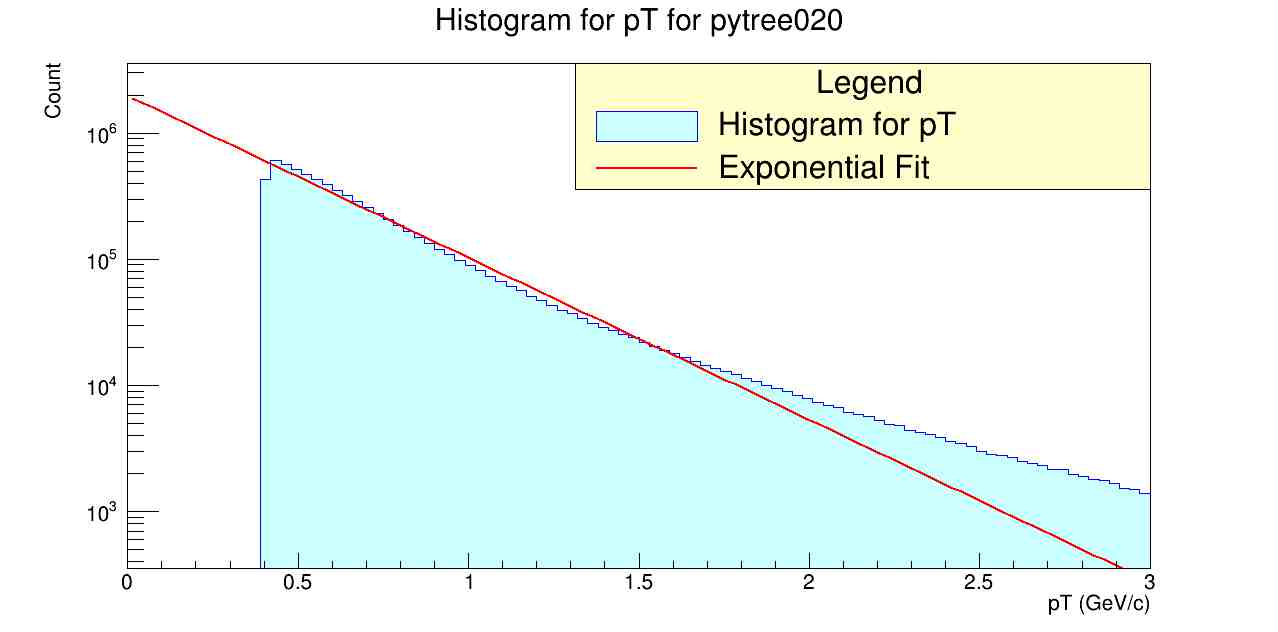
\includegraphics[width=1.1\linewidth]{pt_020}
     \caption{(Color Online) Distribution of $\mathbf{pT}$ for proton-proton collision in the multiplicity class \textbf{pytree020}. The solid line is an Exponential fit to the data. Owing to the large size of the data, the data has been arranged in a random order and only the first \textbf{40\%} of the data has been used for analysis.}
   \end{minipage}\hfill
   \begin{minipage}{0.48\textwidth}
     \centering
     \renewcommand{\thefigure}{1b}
     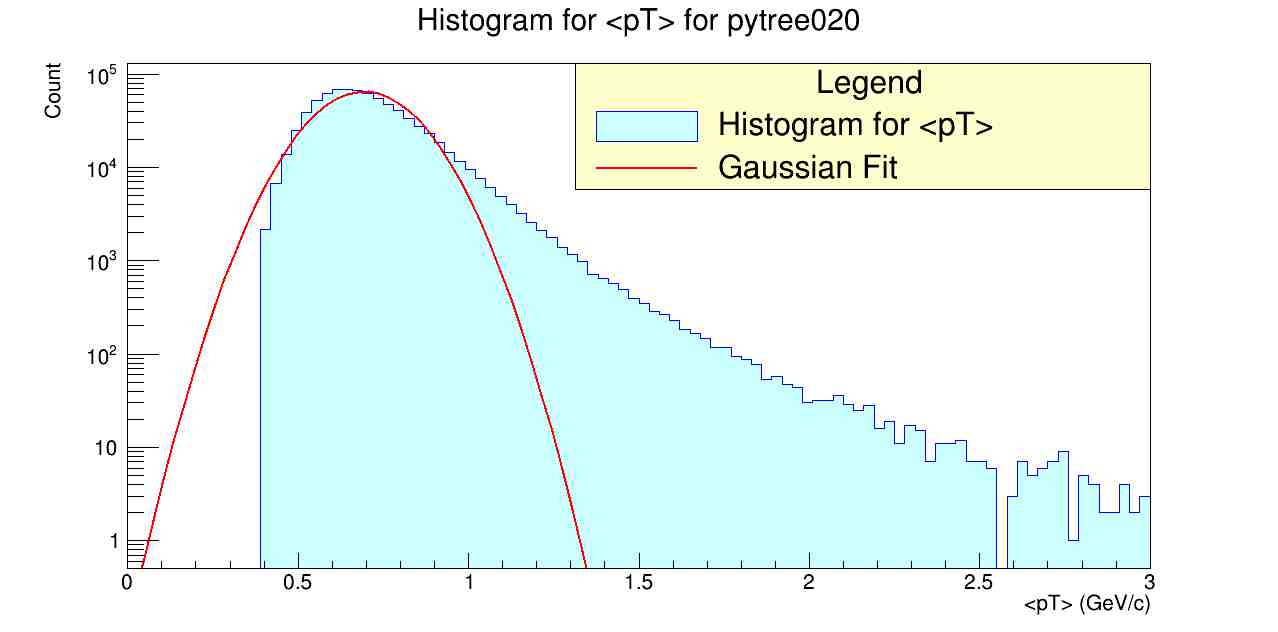
\includegraphics[width=1.1\linewidth]{/mpt_020}
     \caption{(Color Online) Distribution of $\mathbf{\langle pT\rangle }$ for proton-proton collision in the multiplicity class \textbf{pytree020}. The solid line is a Gaussian fit to the data. Owing to the large size of the data, the data has been arranged in a random order and only the first \textbf{40\%} of the data has been used for analysis.}
   \end{minipage}
\end{figure}

\FloatBarrier
\vspace{-3mm}
\pagebreak



\subsubsection{Multiplicity Class "pytree2040"}
\label{subsubsec:2040}
\vspace{-5mm}
\begin{figure}[!htb]
   \begin{minipage}{0.48\textwidth}
   \label{Fig:2a}
   \label{Fig:2b}
     \centering
     \renewcommand{\thefigure}{2a}
     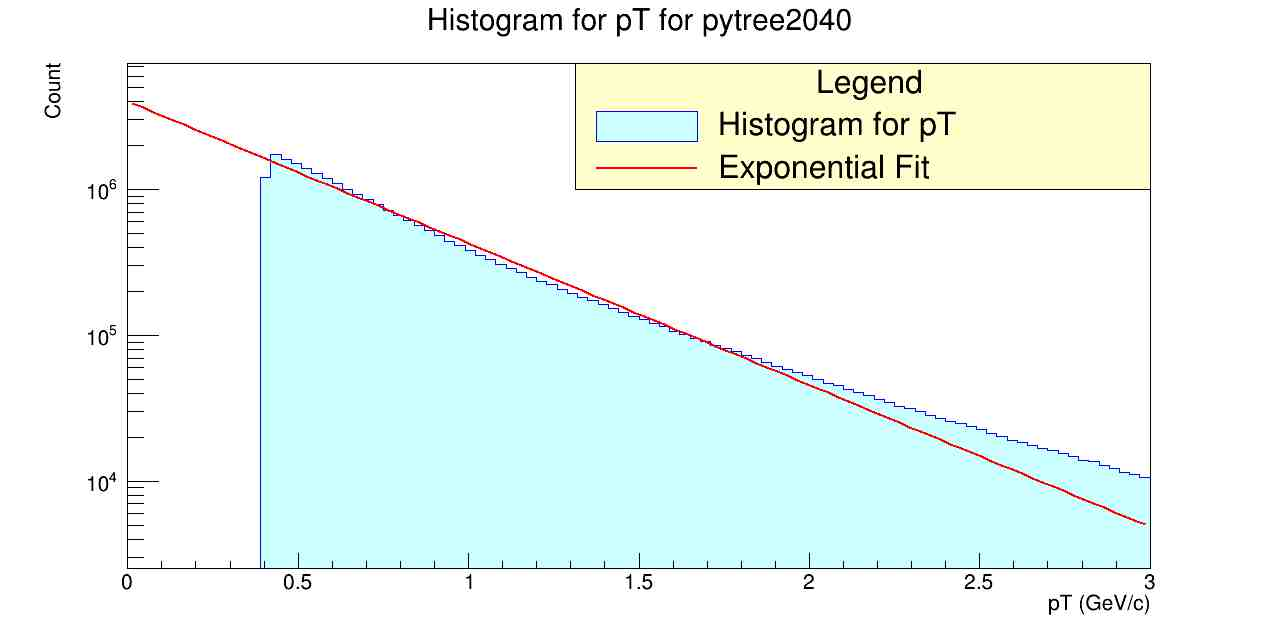
\includegraphics[width=1.1\linewidth]{pt_2040}
     \caption{(Color Online) Distribution of $\mathbf{pT}$ for proton-proton collision in the multiplicity class \textbf{pytree2040}. The solid line is an Exponential fit to the data.}
   \end{minipage}\hfill
   \begin{minipage}{0.48\textwidth}
     \centering
     \renewcommand{\thefigure}{2b}
     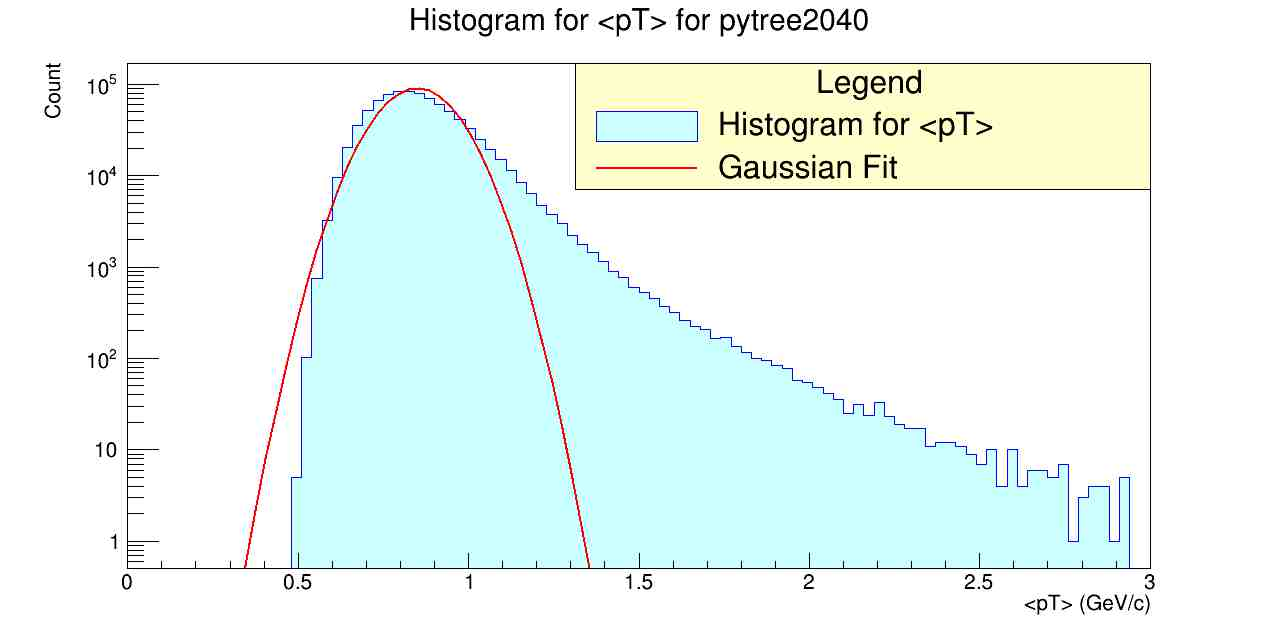
\includegraphics[width=1.1\linewidth]{/mpt_2040}
     \caption{(Color Online) Distribution of $\mathbf{\langle pT\rangle }$ for proton-proton collision in the multiplicity class \textbf{pytree2040}. The solid line is a Gaussian fit to the data.}
   \end{minipage}
\end{figure}

\FloatBarrier
\vspace{-3mm}
%\pagebreak

\subsubsection{Multiplicity Class "pytree4060"}
\label{subsubsec:4060}
\vspace{-5mm}
\begin{figure}[!htb]
   \begin{minipage}{0.48\textwidth}
   \label{Fig:3a}
   \label{Fig:3b}
     \centering
     \renewcommand{\thefigure}{3a}
     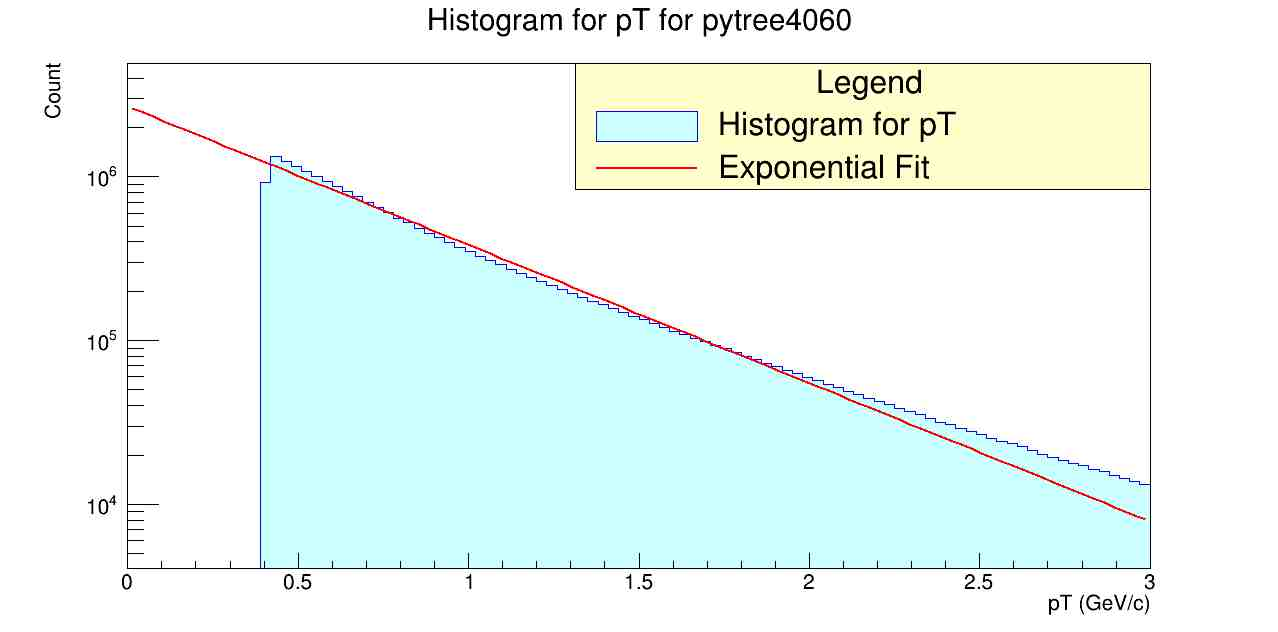
\includegraphics[width=1.1\linewidth]{pt_4060}
     \caption{(Color Online) Distribution of $\mathbf{pT}$ for proton-proton collision in the multiplicity class \textbf{pytree4060}. The solid line is an Exponential fit to the data.}
   \end{minipage}\hfill
   \begin{minipage}{0.48\textwidth}
     \centering
     \renewcommand{\thefigure}{3b}
     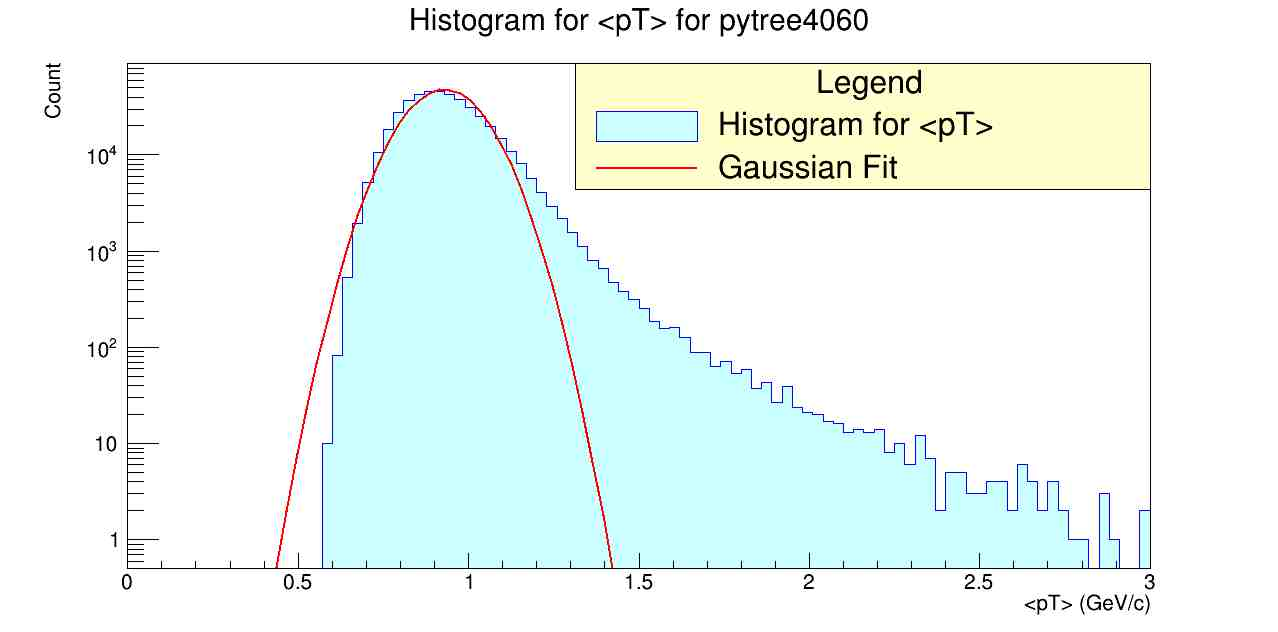
\includegraphics[width=1.1\linewidth]{/mpt_4060}
     \caption{(Color Online) Distribution of $\mathbf{\langle pT\rangle }$ for proton-proton collision in the multiplicity class \textbf{pytree4060}. The solid line is a Gaussian fit to the data.}
   \end{minipage}
\end{figure}

\FloatBarrier
\vspace{-3mm}

\subsubsection{Multiplicity Class "pytree6080"}
\label{subsubsec:6080}
\vspace{-5mm}
\begin{figure}[!htb]
   \begin{minipage}{0.48\textwidth}
   \label{Fig:4a}
   \label{Fig:4b}
     \centering
     \renewcommand{\thefigure}{4a}
     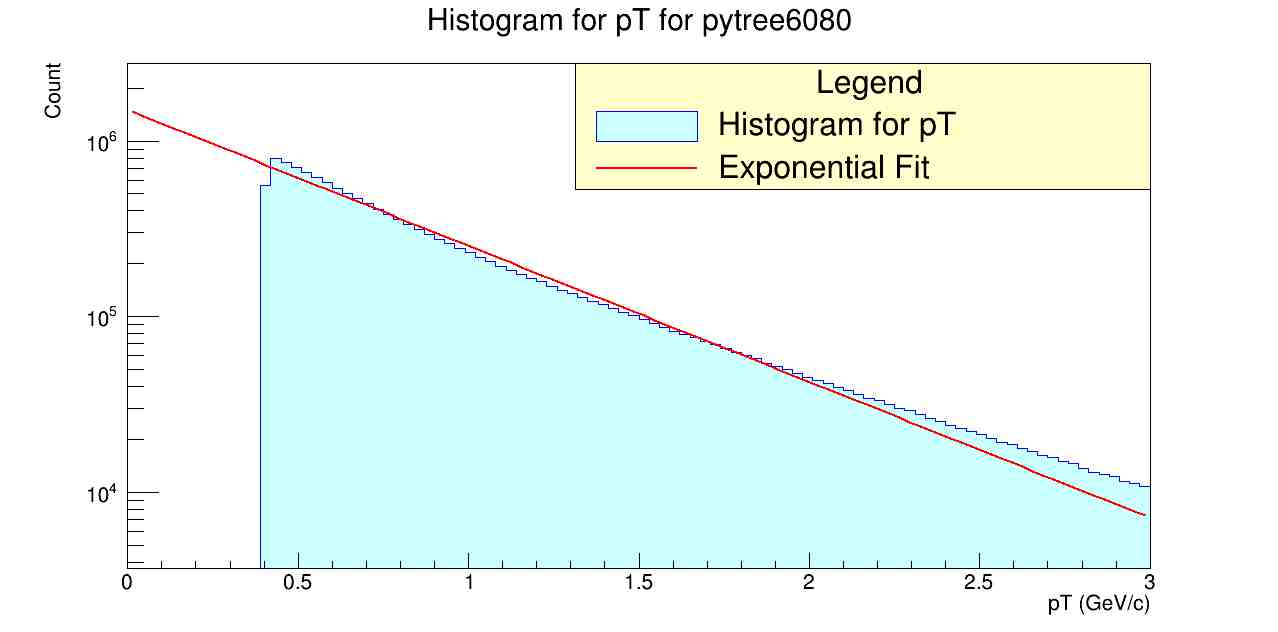
\includegraphics[width=1.1\linewidth]{pt_6080}
     \caption{(Color Online) Distribution of $\mathbf{pT}$ for proton-proton collision in the multiplicity class \textbf{pytree6080}. The solid line is an Exponential fit to the data.}
   \end{minipage}\hfill
   \begin{minipage}{0.48\textwidth}
     \centering
     \renewcommand{\thefigure}{4b}
     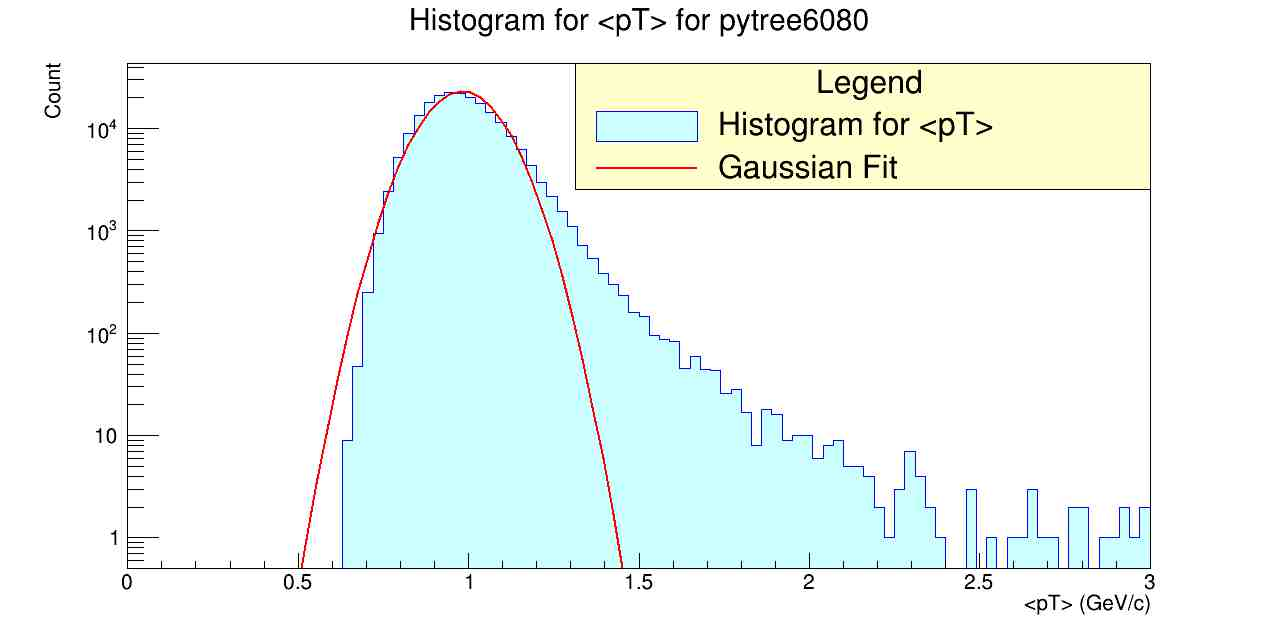
\includegraphics[width=1.1\linewidth]{/mpt_6080}
     \caption{(Color Online) Distribution of $\mathbf{\langle pT\rangle }$ for proton-proton collision in the multiplicity class \textbf{pytree6080}. The solid line is a Gaussian fit to the data.}
   \end{minipage}
\end{figure}

\FloatBarrier
\vspace{-3mm}

\subsubsection{Multiplicity Class "pytree80100"}
\label{subsubsec:80100}
\vspace{-5mm}
\begin{figure}[!htb]
   \begin{minipage}{0.48\textwidth}
   \label{Fig:5a}
   \label{Fig:5b}
     \centering
     \renewcommand{\thefigure}{5a}
     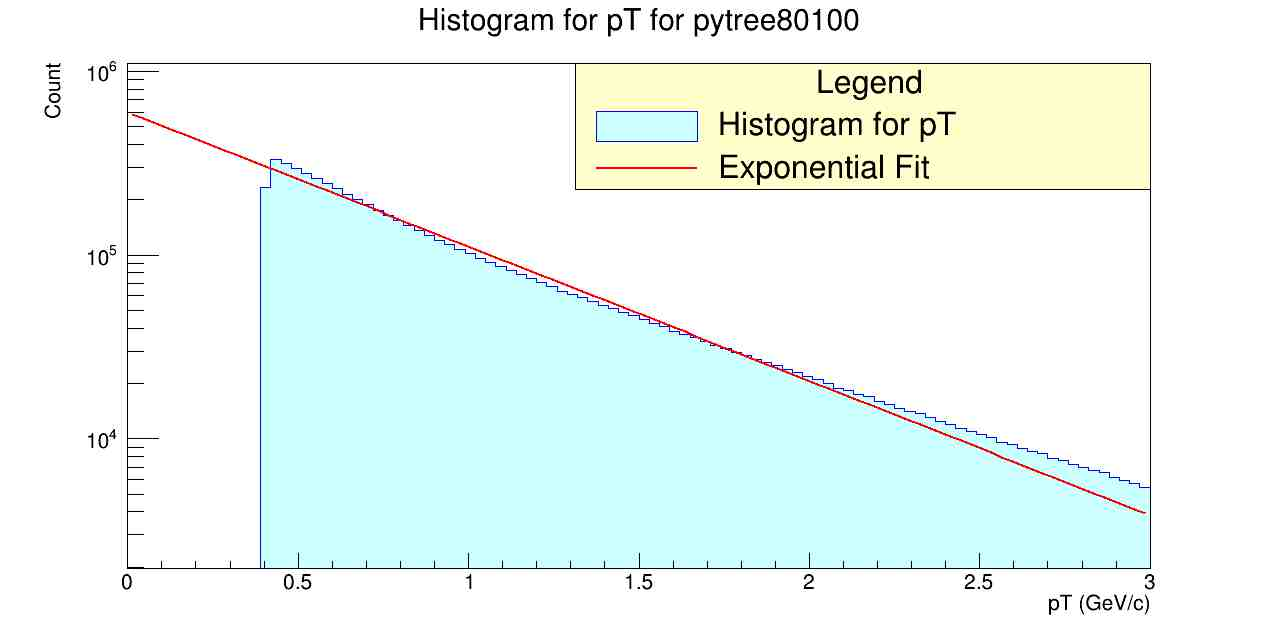
\includegraphics[width=1.1\linewidth]{pt_80100}
     \caption{(Color Online) Distribution of $\mathbf{pT}$ for proton-proton collision in the multiplicity class \textbf{pytree80100}. The solid line is an Exponential fit to the data.}
   \end{minipage}\hfill
   \begin{minipage}{0.48\textwidth}
     \centering
     \renewcommand{\thefigure}{5b}
     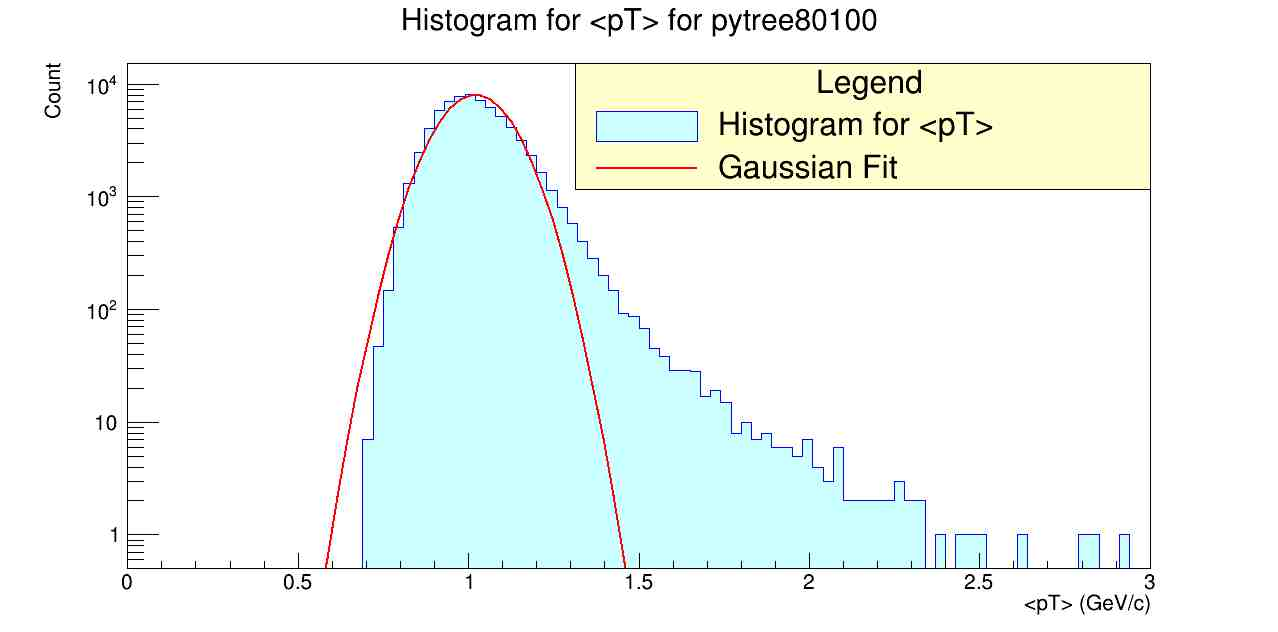
\includegraphics[width=1.1\linewidth]{/mpt_80100}
     \caption{(Color Online) Distribution of $\mathbf{\langle pT\rangle }$ for proton-proton collision in the multiplicity class \textbf{pytree80100}. The solid line is a Gaussian fit to the data.}
   \end{minipage}
\end{figure}

\FloatBarrier
\vspace{-3mm}

\subsubsection{Multiplicity Class "pytree100"}
\label{subsubsec:100}
\vspace{-5mm}
\begin{figure}[!htb]
   \begin{minipage}{0.48\textwidth}
   \label{Fig:6a}
   \label{Fig:6b}
     \centering
     \renewcommand{\thefigure}{6a}
     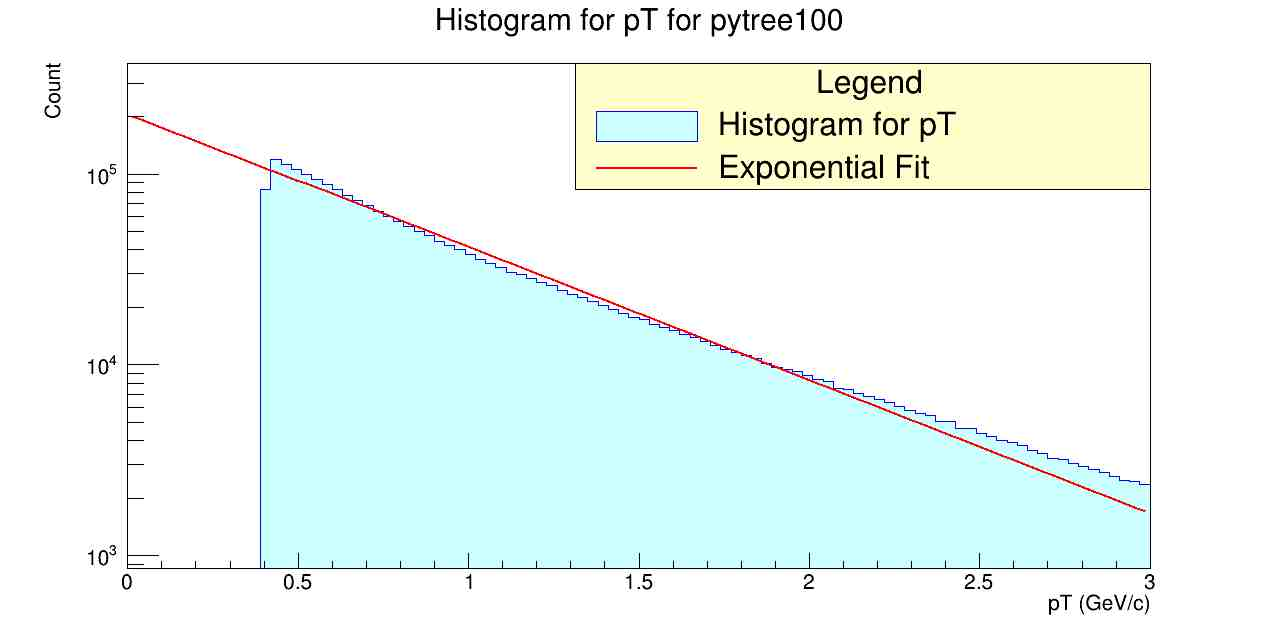
\includegraphics[width=1.1\linewidth]{pt_100}
     \caption{(Color Online) Distribution of $\mathbf{pT}$ for proton-proton collision in the multiplicity class \textbf{pytree100}. The solid line is an Exponential fit to the data.}
   \end{minipage}\hfill
   \begin{minipage}{0.48\textwidth}
     \centering
     \renewcommand{\thefigure}{6b}
     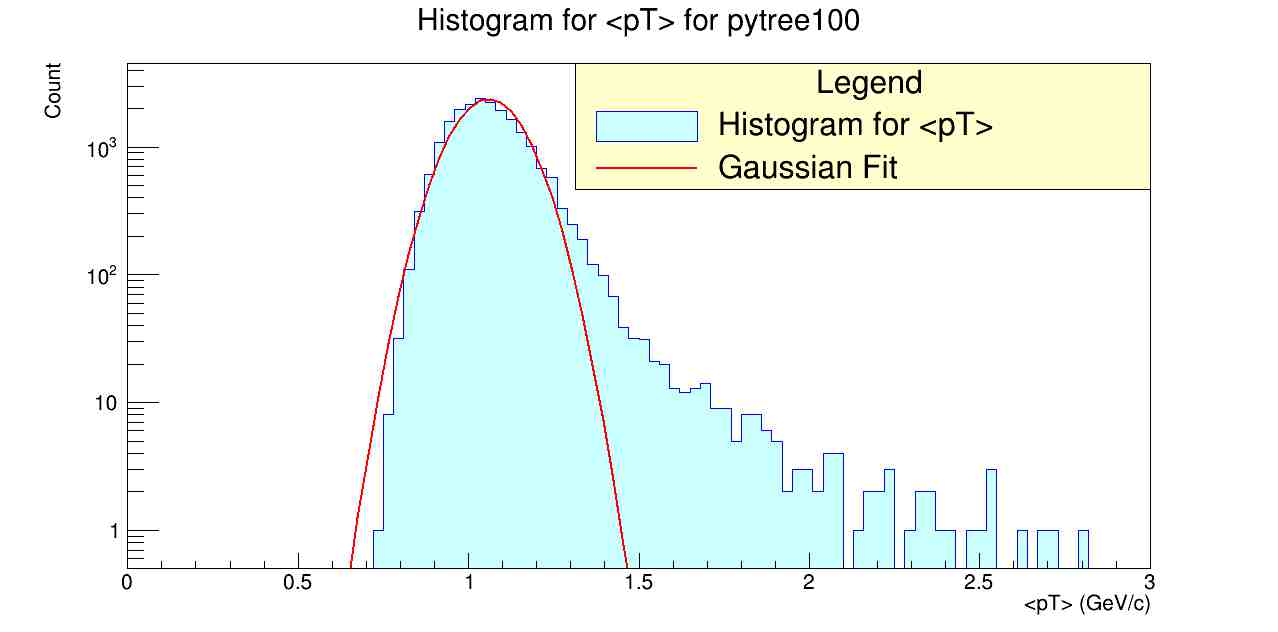
\includegraphics[width=1.1\linewidth]{/mpt_100}
     \caption{(Color Online) Distribution of $\mathbf{\langle pT\rangle }$ for proton-proton collision in the multiplicity class \textbf{pytree100}. The solid line is a Gaussian fit to the data.}
   \end{minipage}
\end{figure}

\FloatBarrier

\subsection{Analysis of Mean, Variance and Skewness Versus Multiplicity Class}
From the graphs in \hyperref[Fig:1a]{FIG. 1a.}, \hyperref[Fig:2a]{FIG. 2a.}, \hyperref[Fig:3a]{FIG. 3a.}, \hyperref[Fig:4a]{FIG. 4a.}, \hyperref[Fig:5a]{FIG. 5a.} and \hyperref[Fig:6a]{FIG. 6a.}, it is clear that the Transverse Momenta of the particles produced in a proton-proton collision follows approximately an \textbf{exponential distribution}. Graphs in \hyperref[Fig:1b]{FIG. 1b.}, \hyperref[Fig:2b]{FIG. 2b.}, \hyperref[Fig:3b]{FIG. 3b.}, \hyperref[Fig:4b]{FIG. 4b.}, \hyperref[Fig:5b]{FIG. 5b.} and \hyperref[Fig:6b]{FIG. 6b.} reveal that there is some \textbf{positive skew} in the distribution of the Mean Transverse Momentum.
\\
In this section, we shall analyse the moments of the distribution of Transverse Momentum. We shall calculate the Mean, Variance and Skewness of the Transverse Momenta for each multiplicity class and study its relation with the multiplicity class. For each of the multiplicity classes, the Mean Transverse Momentum, the Intensive Variance of the Transverse Momentum, the Standardized Skewness of the Transverse Momentum and the Intensive Skewness of the Transverse Momentum, calculated using formulae \ref{eq:1}, \ref{eq:4}, \ref{eq:7} and \ref{eq:8} respectively have been summarised in the \hyperref[subsubsec:summary]{table} and the \hyperref[subsubsec:mean]{plots} below. Note that for \textit{pytree2040}, the number of events is too large for a personal computer at today's scale to handle. Hence, the dataset of this multiplicity class has been randomized and the first \textbf{40\%} has been used for analysis.

\pagebreak
%\newpage

\subsubsection{Summary of Data}
\label{subsubsec:summary}
\vspace{-5mm}
The table below summarizes the data.
\begin{table}[!htb]
\centering
	\begin{tabular}{|M{5cm}|M{2cm}|M{2cm}|M{2cm}|M{2cm}|M{2cm}|}
		\hline
		\multicolumn{6}{|c|}{\addmathvspace\textbf{SUMMARY OF DATA}}\\
		\hline
		\addmathvspace\textbf{Multiplicity Class} & 
		$\mathbf{Events}$ & 
		\begin{tabular}{c}
			$\large\mathbf{\langle p_T\rangle }$\\[2pt]
			\textbf{(GeV/c)}
		\end{tabular} &
		$\large\mathbf{\sigma_{p_T}}$ & 
		\begin{tabular}{c}
			$\large\mathbf{\gamma_{p_T}}$\\[2pt]
			\textbf{(GeV/c)}
		\end{tabular} &		 
		$\large\mathbf{\Gamma_{p_T}}$\\[5pt]
		\hline
		\textit{pytree020}&\addmathvspace952256&0.750912&0.235453&1.22572&5.20581\\[3pt]
		\hline
		\textit{pytree2040}&\addmathvspace873322&0.869307&0.174974&1.77742&10.1582\\[3pt]
		\hline
		\textit{pytree4060}&\addmathvspace445805&0.940521&0.144591&1.80884&12.51\\[3pt]
		\hline
		\textit{pytree6080}&\addmathvspace207990&0.99074&0.130471&3.11451&23.8714\\[3pt]
		\hline
		\textit{pytree80100}&\addmathvspace71263&1.03006&0.122603&1.64507&13.4178\\[3pt]
		\hline
		\textit{pytree100}&\addmathvspace20981&1.07257&0.132207&4.11805&31.1485\\[5pt]
		\hline		
	\end{tabular}
	\caption{Table Summarizing the Data of Transverse Momenta}
\end{table}

\FloatBarrier
\subsubsection{Mean Transverse Momentum versus Multiplicity Class}
\label{subsubsec:mean}
\vspace{-5mm}
\begin{figure}[!htb]
	\begin{minipage}{1\textwidth}
   		\label{Fig:6}
     	\centering
     	\renewcommand{\thefigure}{6}
     	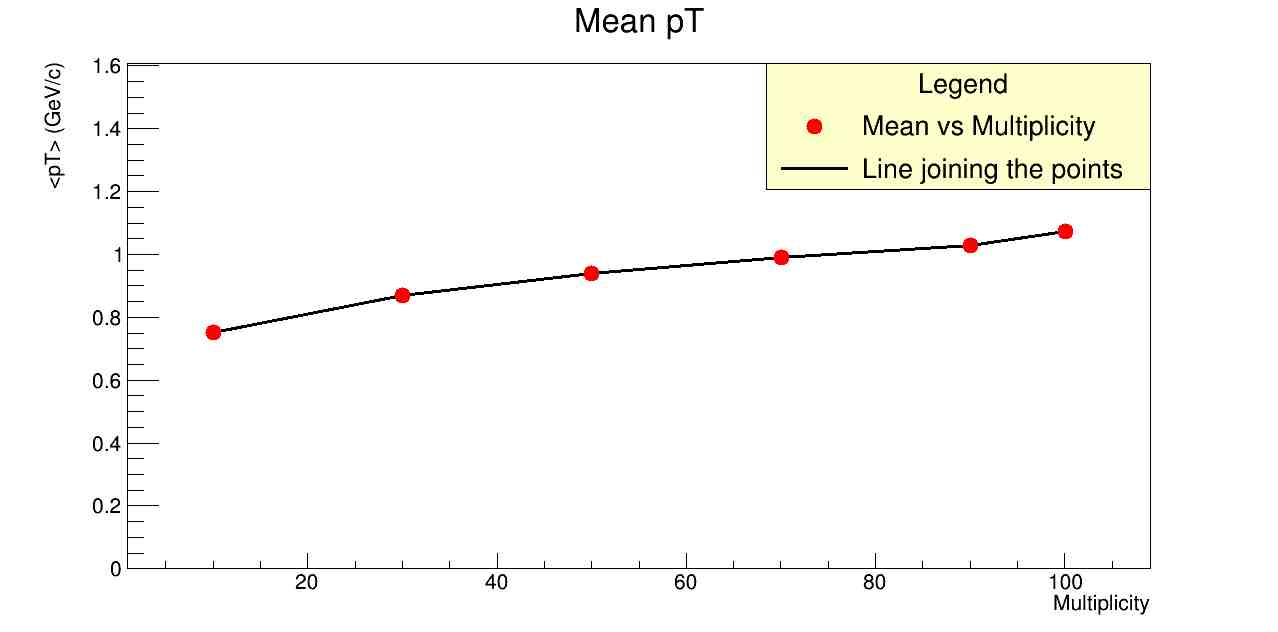
\includegraphics[width=\linewidth]{mean}
     	\begin{minipage}{0.8\textwidth}
     	\caption{(Color Online) A plot of \textbf{mean} transverse momenta versus multiplicity class. The red dots represent the mean of the transverse momentum. The solid line shows the trend of the mean against the multiplicity class.}
     	\end{minipage}
     \end{minipage}
\end{figure}

\FloatBarrier
\vspace{-3mm}


\subsubsection{Intensive Variance of Transverse Momentum versus Multiplicity Class}
\label{subsubsec:intvar}
\vspace{-5mm}
\begin{figure}[!htb]
\begin{minipage}{\textwidth}
   \label{Fig:7}
     \centering
     \renewcommand{\thefigure}{7}
     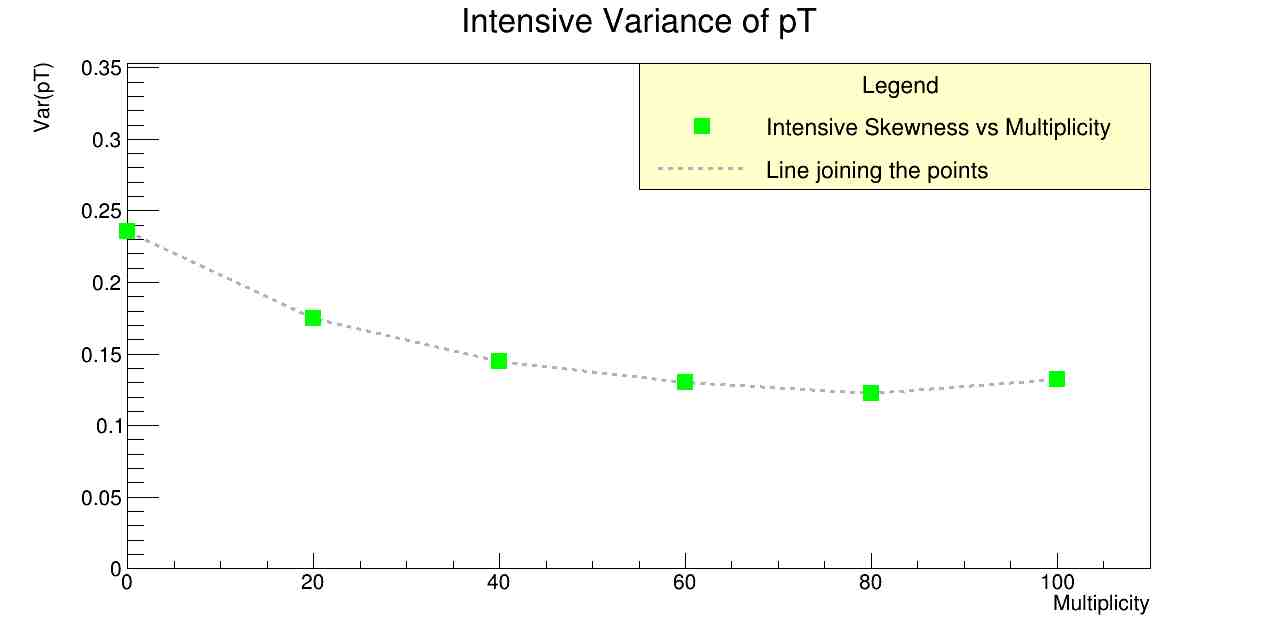
\includegraphics[width=\linewidth]{intvar}
     \begin{minipage}{0.8\textwidth}
     \caption{(Color Online) A plot of the \textbf{intensive variance} of transverse momenta versus multiplicity class. The green boxes represent the intensive variance of the transverse momentum. The dashed line shows the trend of the intensive variance against the multiplicity class.}
     \end{minipage}
\end{minipage}
\end{figure}

\FloatBarrier
\vspace{-3mm}

\subsubsection{Standardized Skewness of Transverse Momentum versus Multiplicity Class}
\label{subsubsec:stdskew}
\vspace{-5mm}
\begin{figure}[!htb]
\begin{minipage}{\textwidth}
   \label{Fig:8}
     \centering
     \renewcommand{\thefigure}{8}
     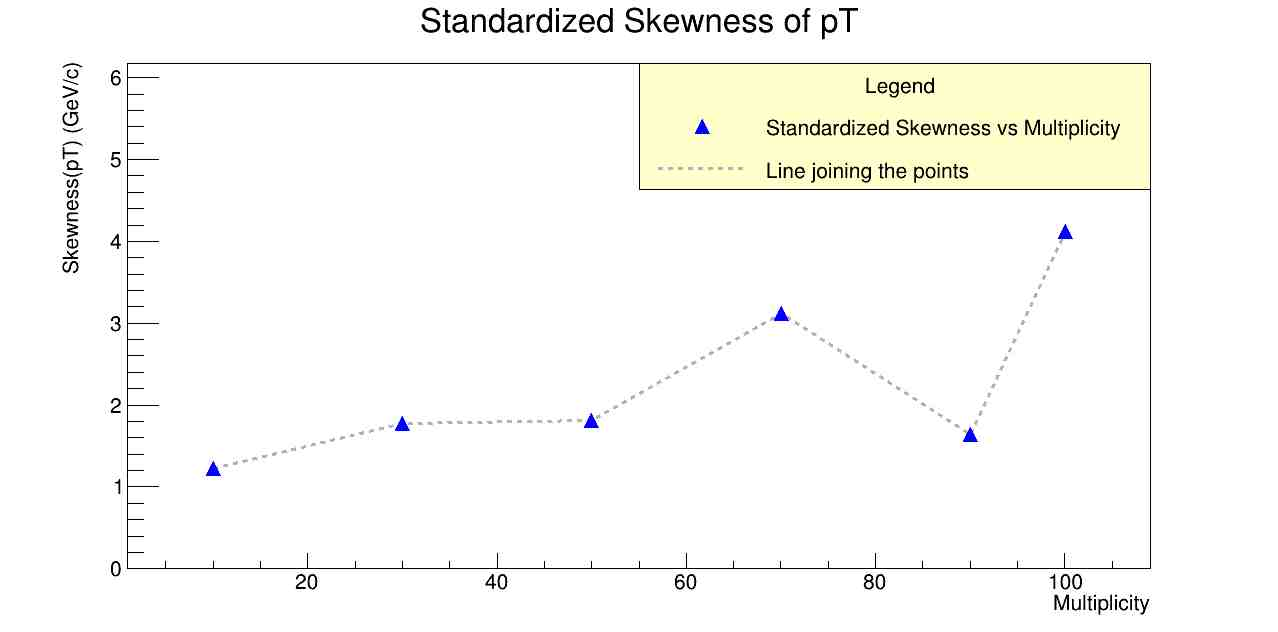
\includegraphics[width=\linewidth]{stdskew}
     \begin{minipage}{0.8\textwidth}
     \caption{(Color Online) A plot of the \textbf{standardized skewness} of transverse momenta versus multiplicity class. The blue triangles represent the standardized skewness of the transverse momentum. The dashed line shows the trend of the standardized skewness against the multiplicity class.}
     \end{minipage}     
\end{minipage}
\end{figure}

\FloatBarrier
\vspace{-1mm}

\subsubsection{Intensive Skewness of Transverse Momentum versus Multiplicity Class}
\label{subsubsec:intskew}
\vspace{-5mm}
\begin{figure}[!htb]
\begin{minipage}{\textwidth}
   \label{Fig:9}
     \centering
     \renewcommand{\thefigure}{9}
     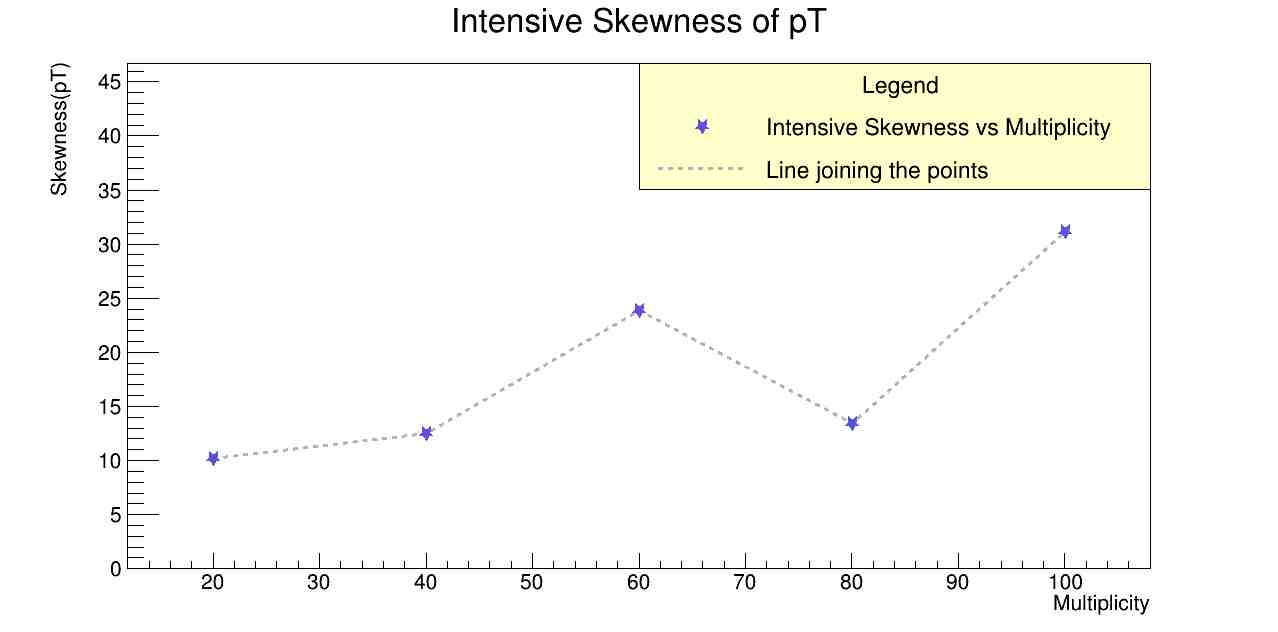
\includegraphics[width=\linewidth]{intskew}
     \begin{minipage}{0.8\textwidth}
     \caption{(Color Online) A plot of the \textbf{intensive skewness} of transverse momenta versus multiplicity class. The cyan stars represent the intensive skewness of the transverse momentum. The dashed line shows the trend of the intensive skewness against the multiplicity class.}
     \end{minipage}
     
\end{minipage}
\end{figure}



\vspace{-2mm}


\section{Summary}
\vspace{-2mm}
The fluctuations occurring in the mean transverse momentum $\mathbf{\langle p_T\rangle }$ of emitted particles in various collisions have several underlying causes. We have shown that the various statistical and dynamical fluctuations are being reflected on the distribution of $\mathbf{\langle p_T\rangle }$. It is very clear that the function of $\mathbf{\langle p_T\rangle }$ versus collision count tends to have a \textbf{positive skewness in Gaussian fit}. Hydrodynamics predicts that the event-by-event fluctuations of the mean transverse momentum, $\mathbf{\langle p_T\rangle }$, have positive skew. The fluctuation can be calculated in terms of standardized skewness and intensive skewness. At the centre of mass energy \textbf{13 TeV} for \textbf{p+p collision}, the standardized skewness tends to have values between \textbf{1.2 to 4.2 GeV/c} and intensive skewness has values between \textbf{5.2 to 31.2} for corresponding multiplicity classes. From \hyperref[subsubsec:mean]{FIG. 6.}, we conclude that the mean transverse momentum is \textbf{monotonically increasing} with respect to the multiplicity class. \hyperref[subsubsec:intvar]{FIG. 7.} shows that the intensive variance of transverse momentum is \textbf{monotonically decreasing} with respect to the multiplicity class. From the graphs in \hyperref[subsubsec:stdskew]{FIG. 8.} and \hyperref[subsubsec:intskew]{FIG. 9.}, it is evident that both standardized as well as intensive skewness of transverse momentum \textbf{increases} with multiplicity class, with one exception. For the multiplicity class \textit{pytree80100} it shows a dip in value of skewness. This could be for several reasons. Some of them are mentioned below.
\begin{enumerate}[label=(\roman*)]
\itemsep0em
\item The events are simulated using a Monte Carlo Generator, which in some extreme cases produce data sets that are very close to the mean (having very few outliers)
\item The number of events in \textit{pytree80100} is much less than the previous multiplicity classes, as seen from the \hyperref[subsubsec:summary]{table}
\item As seen from \hyperref[Fig:5b]{FIG. 5b.}, the histogram of the distribution of $\mathbf{\langle p_T\rangle }$ has a steep decreasing slope towards the right, which is indicative of higher resemblance to a Gaussian fit. This might occur due to the finite size of the data. 
\end{enumerate}
Needless to say, the origin and the behaviour of the skewness is a deep and interesting topic that requires further discussion in near future.



\begin{thebibliography}{50}
\medskip


%\bibitem{phenixwhite} K. ~Adcox 
  %Nuclear Phys. A{\bf 757},184-283 (2005). 
  

%\bibitem{fluct} J. ~Adams {\it et al.}, (ALICE Collaboration), Nature Physics{\bf 13},535-539 (2017). 
\bibitem{fluct}  Giuliano Giacalone {\it et al.}, \textit{Skewness of mean transverse momentum fluctuations in heavy-ion collisions} (arXiv:2004.09799 [nucl-th])

\end{thebibliography}

\end{document}

